\documentclass[11pt, aspectratio=169, xcolor=table]{beamer}
\usepackage[utf8]{inputenc}
\usepackage[T1]{fontenc}
\usepackage{graphicx}
\usepackage{hyperref}
\usepackage{lmodern}
\usepackage[spanish]{babel}
\usepackage{pdfrender}
\usepackage{xcolor}
\usepackage{ragged2e}
\usepackage[version=4]{mhchem}
\usepackage{siunitx}
\renewcommand{\raggedright}{\justifying}
\usepackage{smartdiagram}
\usetheme{Berlin}

\author{Prof. Daniel Muñoz \\
	\texttt{daniel.munoz3@mail.udp.cl}
}
\title{Química Unidad 3}
\subtitle{Del caos molecular a sistemas en equilibrio}
\titlegraphic{\includegraphics[width=4cm]{../img/udplogo}}

\begin{document}

\maketitle

\section[TCM: PVNT]{Teoría cinético molecular y variables de estado}
\begin{frame}[allowdisplaybreaks]
	\frametitle{Ludwing Boltzman: 1844 - 1906}
	\begin{columns}
		\begin{column}{.5\textwidth}
			\begin{itemize}
				\scriptsize
				\item Físico Austriaco padre de la mecánica estadística.
				\item Desarrollo el concepto actualmente usado de entropía.
				\item Logró vincular propiedades macroscópicas con microscópicas mediante tratamientos estadísticos.
				\item Sus trabajos fueron continuados posteriormente por Einstein y defendidos por Planck.
				\item En 1906 se suicida, según mencionan, por falta de reconocimiento.
			\end{itemize}
		\end{column}

		\begin{column}{.5\textwidth}
			\begin{figure}[ht]
				\centering
				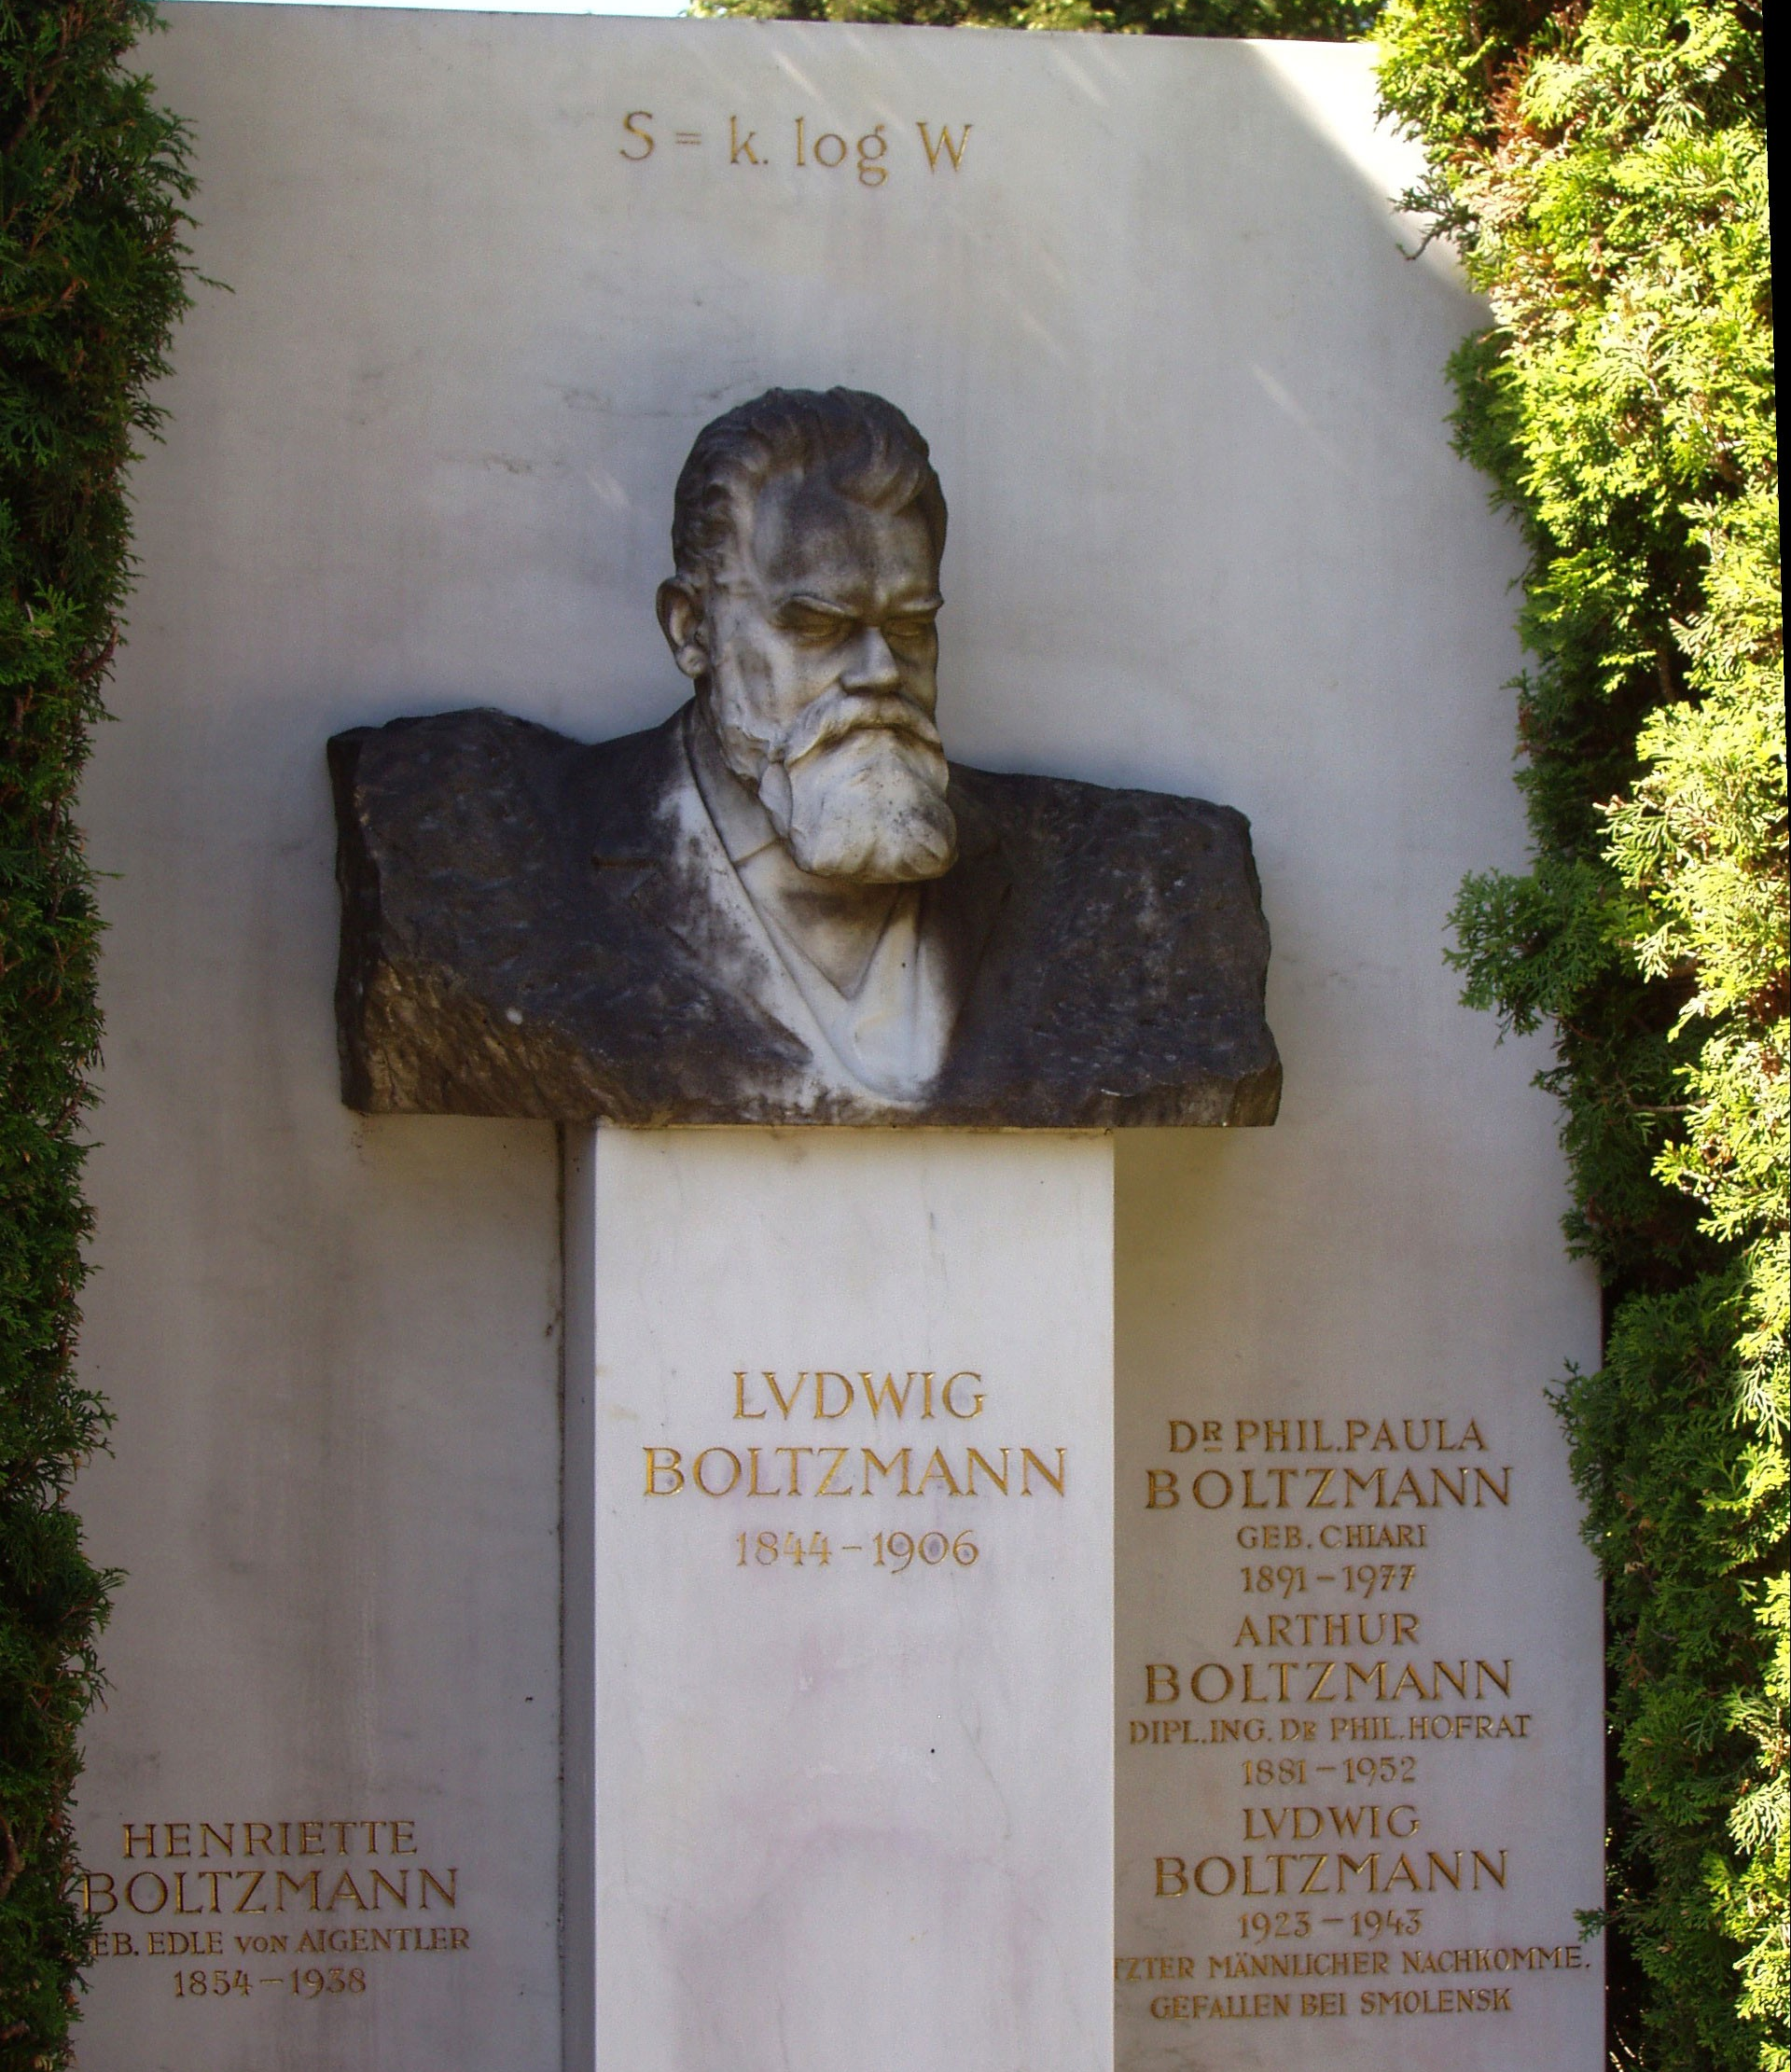
\includegraphics[height=0.6\textheight]{../img/boltzman.png}
				\caption{\label{fig:label} Tumba de Boltzman en Viena}
			\end{figure}

		\end{column}
	\end{columns}
\end{frame}

\begin{frame}
  \frametitle{Teoría Cinético Molecular (TCM)}
  \begin{columns}
    \begin{column}{0.5\textwidth}
      \begin{itemize}
        \footnotesize
        \item Una de las grandes conclusiones de LB es que para predecir el comportamiento de un gas podemos asumir que no poseen estructura interna. 
        \item Esto significa que podemos suponer el mismo comportamiento para un gas monoatómico, que para un gas poliatómico
        \item Esta sencilla, pero poderosa observación nos permite predecir un gas conocimiento muy pocos elementos de él.
        \item Actualmente sabemos que eso es cierto bajo ciertas condiciones P $\approx$ \qty{1}{atm} y T < \qty{30}{\degreeCelsius}
      \end{itemize}
    \end{column}
    \begin{column}{0.5\textwidth}
      \begin{figure}[ht]
        \centering
        \includegraphics[width=\textwidth]{../img/billar.jpg}
        \caption{El billar es un ejemplo de como se comporta todo gas ``ideal''}
        \label{fig:2}
      \end{figure}
    \end{column}
  \end{columns}
\end{frame}

\begin{frame}
  \frametitle{Variables de estado}
  \begin{columns}
    \begin{column}{0.5\textwidth}
      \begin{block}{Variable}
        Magnitud física que cambia. Ejemplo: tiempo.
      \end{block}
    \end{column}
    \begin{column}{0.5\textwidth}
      \begin{block}{Estado}
        Todas las variables que describen un sistema (gas).
      \end{block}
    \end{column}
  \end{columns}
\end{frame}


\section[Leyes de los gases]{Leyes de los gases: Boyle, Charles, Gay-Lussac y Avogadro}

\begin{frame}[allowdisplaybrakes]
  \frametitle{Ley de Boyle-Mariotte}
  
\end{frame}

\begin{frame}
  \frametitle{Ley de Charles}
  
\end{frame}

\begin{frame}
  \frametitle{Ley Gay-Lussac}
  
\end{frame}

\begin{frame}
  \frametitle{Ley de Avogadro}
  
\end{frame}
\section{Aplicación de la Ley de los gases ideales}

\section{Cálculos estequimétricos en gases ideales}

\begin{frame}
  \frametitle{Bibliografía}
  \begin{thebibliography}{99}
    \setbeamertemplate{bibliography item}[book]
    \bibitem[Chang, 2011]{Chang2011}
    Chang, Raymond
    \newblock \emph{Fundamentos de Química}
    \newblock McGraw Hill, 2011
  \end{thebibliography}
\end{frame}

\end{document}
